In Milestone 1, user-space processes were given the ability to obtain physical memory through the capabilities system, and we also implemented a bare-bones virtual address space that could handle very simple mappings. In order to do things like spawn a process (which we do in Milestone 3), we require a full virtual memory system supporting arbitrary mappings and unmappings as well as an MMU-independent, per-process paging system.

\subsection{Design Constraints}
As mentioned above, our user-space processes can now obtain RAM capabilities and retype them into frames. To actually use this memory though, they need to be able to map the frames to virtual addresses. In other words, we want our processes to each be able to use the entire memory space without having to worry about what parts of it are in use by other processes. This implies that we need a mechanism for translating between process memory and actual physical memory (hence why we say ``map physical frames to virtual addresses"). This provides us with a number of benefits such as being able to avoid allocating large chunks of physical memory until necessary, as well as being able to load programs at arbitrary physical locations (even though they were compiled and linked for specific addresses).
\\\\
It is conventionally the job of the MMU to deal with virtual address translation, however since our OS is self-paging, processes explicitly acquire physical memory and then program the MMU with their own constructed page tables. Two main challenges were apparent to our group when we started thinking about a plan of attack for this Milestone:
\begin{enumerate}[itemsep=0pt]
    \item How do we find a free virtual address region to map into? In other words, what per-region metadata needs to be stored and how do we store it?
    \item We need to create page tables for allocated virtual memory space and keep track of their state; how should this be done?
\end{enumerate}
While also fundamental to getting things working, these questions were of particular importance to us since mapping/unmapping operations can easily happen tens of thousands of times during the runtime of an operating system. As such, we were looking for a design that lent itself to quick virtual address region lookups and quick page table lookups/insertions. 

\subsection{Virtual Address Region Layout}
We now describe the first major challenge of this milestone: given a frame, how does a process find an appropriately-sized, free virtual address region to map it to? We need a data structure to maintain the state of virtual address regions. Each region can be free, allocated but not mapped, or allocated and mapped. Some regions will be mapped and physically allocated all at once, e.g. ``eagerly allocated". A region that is virtually allocated but neither mapped nor physically allocated is ``lazily allocated." If a process tries to access the lazily allocated region, a page fault will be triggered and a page of physical memory will be mapped to back the virtual address. In following sections, we will sometimes denote virtual memory allocation as ``reservation" to provide lexical distinction between virtual and physical memory allocation. For this section, we focus on the ``virtual memory manager", which maintains metadata for virtual address regions and determines which regions to allocate on request. Since this problem is almost identical to that of physical memory management in Milestone 1, we must consider the same data structure requirements as we did for the \hyperref[m1-3]{physical memory manager}. In addition to those listed in the referred section, there is an extra detail to account for in virtual memory management:
\begin{itemize}[itemsep=0pt]
    \item Our data structure should be able to represent non-contiguous virtual address ranges (and mark those range as free/allocated).
\end{itemize}

In Milestone 1, physical addresses were not important to physical memory allocation, as processes do not access memory by physical addresses. This is a different case for our virtual memory manager, where we must consider a memory region's address, in addition to its size.

\subsubsection{The Generic Allocator}\label{m2-2}
We started implementing our virtual region memory manager with a simple linked list, just to get things working (we ended up not having the time to swap this out). Each node in the list would represent a reserved region and store data such as its address, size, and whether or not it was mapped. As we have mentioned, since this problem is almost identical to the issue of physical memory management in Milestone 1, we created an interface for our memory manager structures, which we refer to as the ``generic allocator" to reuse some pre-existing functionality.
\\\\
The generic allocator (shown in Figure \ref{figure:m2_diagram}) is an abstract interface that stores a linked list whose nodes each refer to regions of the address space. As an abstract interface, it allows users to add allocator-specific data for regions, errors, functions, and its backing slab allocator. We take advantage of this feature in our virtual memory manager to store extra region data to distinguish between ``reserved" and ``mapped" memory, which we describe in a later section on \hyperref[m2-4]{Heap Memory Management}. 
\\\\
Code for the generic allocator can be found in \texttt{lib/aos/generic\_allocator.c}.
\begin{figure}[ht]
    \centering
    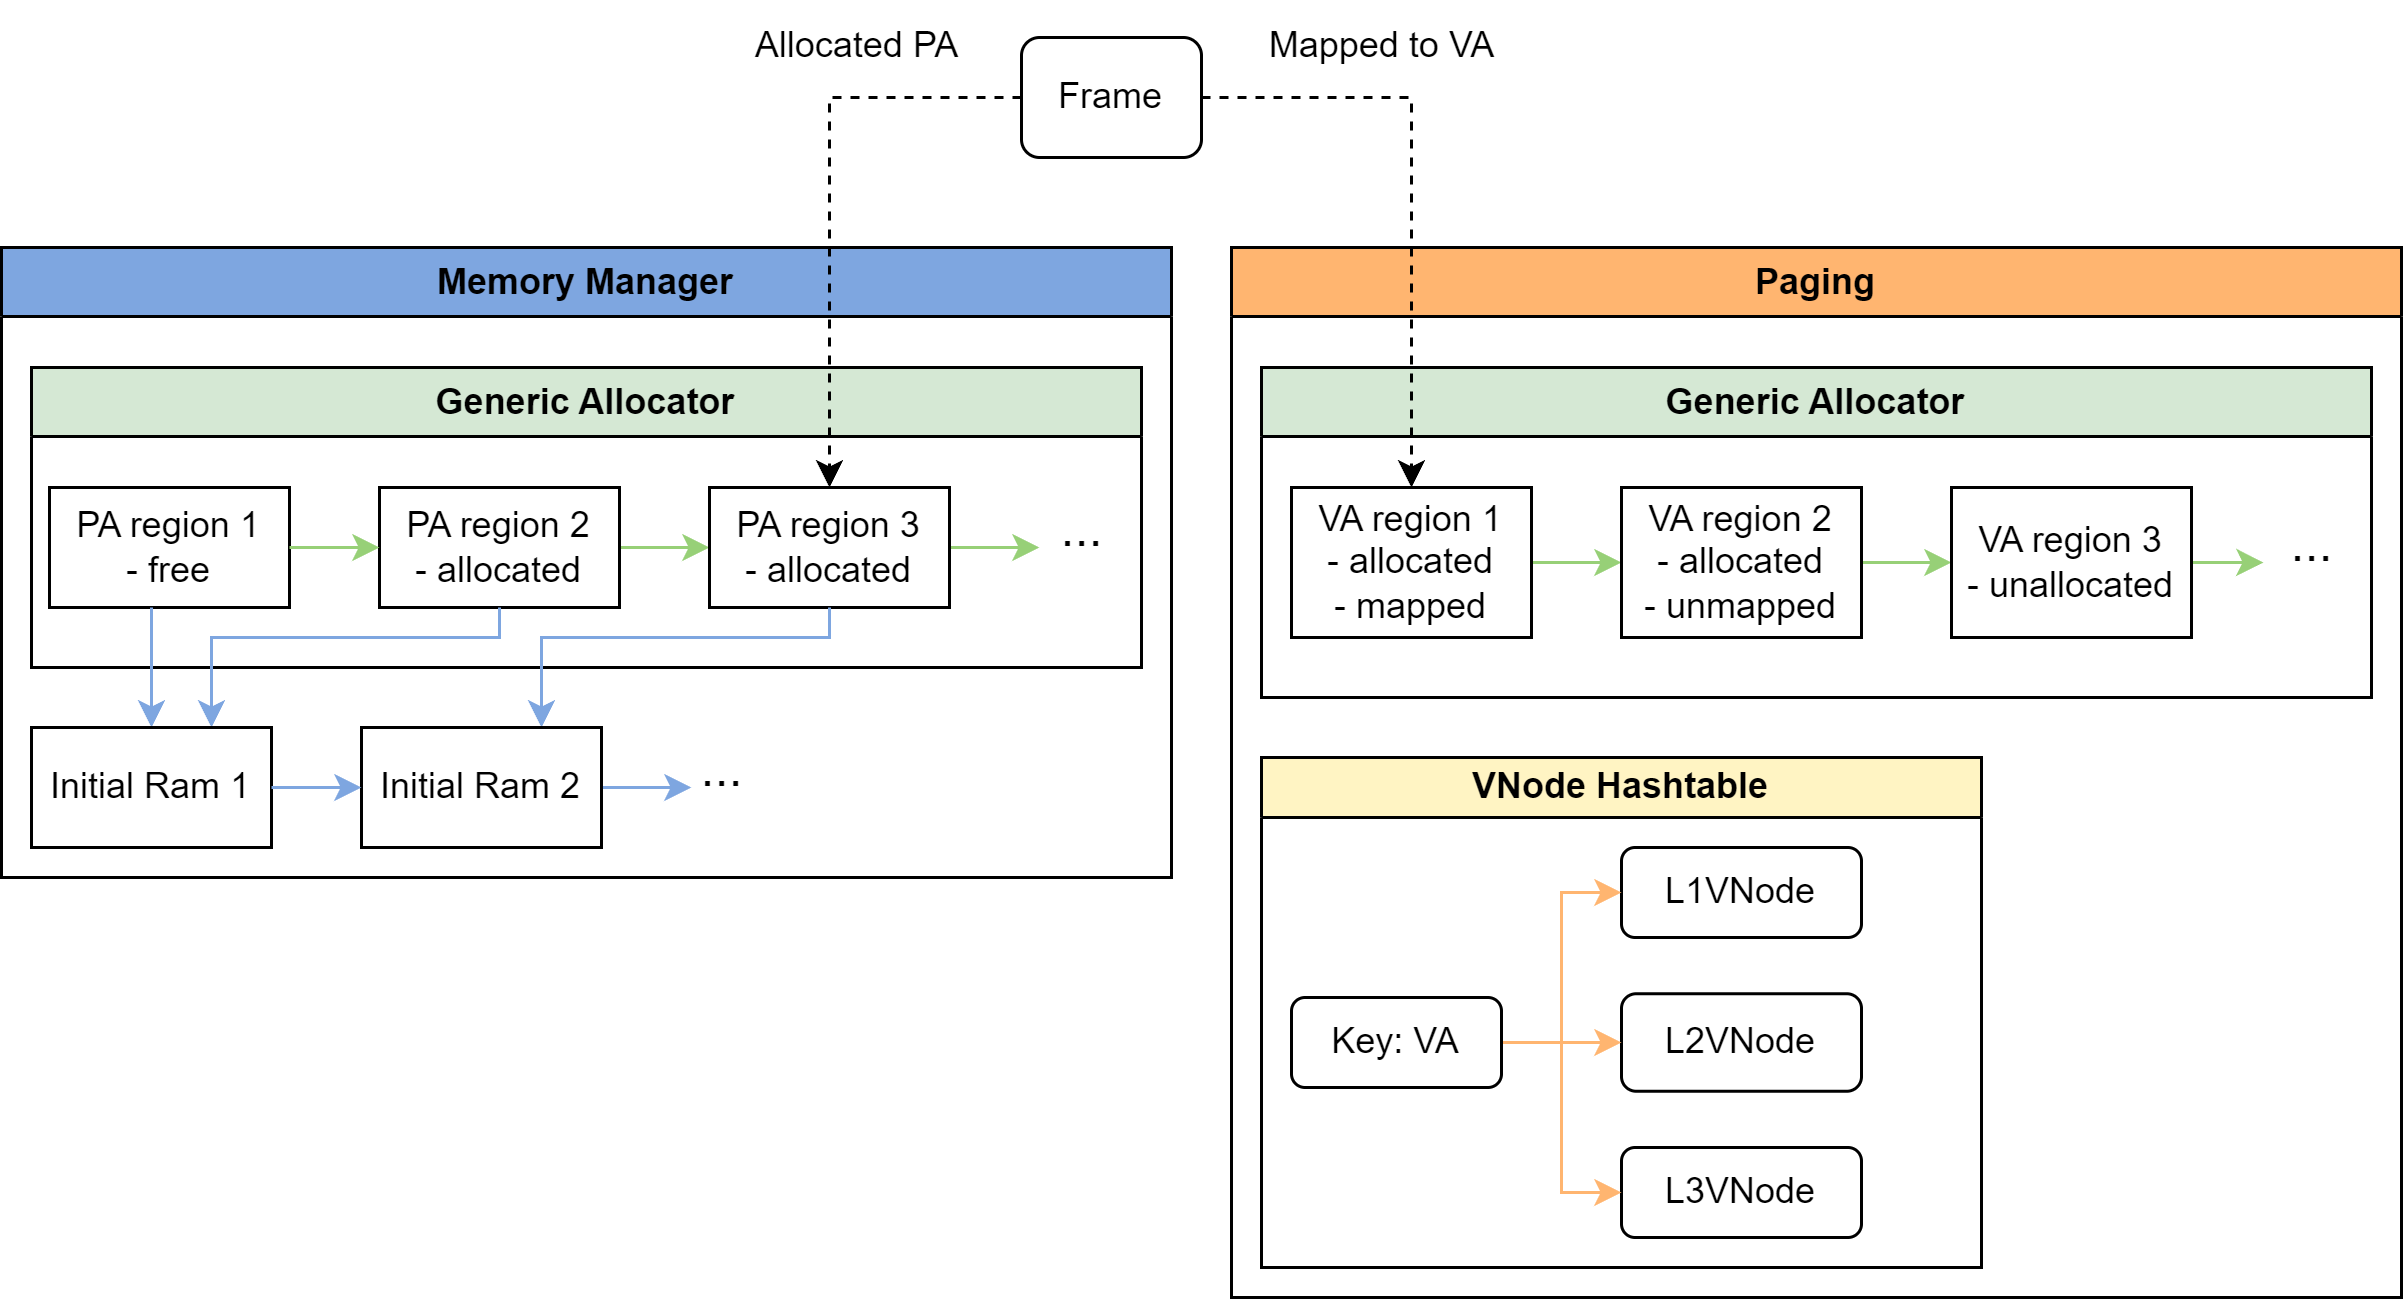
\includegraphics[width=0.8\columnwidth]{images/m2_diagram.png}
    \caption{Usage of the generic allocator in our memory manager and paging implementations.}
    \label{figure:m2_diagram}
\end{figure}
\\\\
The decision to use a linked list, and in particular a ``generic" linked list has been already detailed in \hyperref[m1-2]{Section 2.3.1}. Besides the reasons already described there, the primary benefit of a linked list for the virtual memory manager lies in the fact that a linked list node can easily represent an address range. By storing the starting address and corresponding size of the region in a node, we only require as many nodes as there are allocated regions in our virtual address space, which minimizes the memory overhead by a large margin. In the third point of \hyperref[m1-2]{Section 2.3.1}, we mention that our linked list preserves ordering of the nodes by its base virtual address. This is important to our \texttt{next-fit} allocation strategy, specific to the virtual memory manager. Since we are now concerned with a memory region's addressing during allocation, we do not want an out-of-order list, as \texttt{next-fit} may end up having to walk the entire list in search for an appropriate virtual address to allocate.
\\\\
The alternative data structures detailed in \hyperref[m1-6]{Section 2.6} were also considered for the virtual memory manager and not chosen for the same reasons.
An additional alternative data structure we considered for the task of virtual address region management was a hash table. Using a hash table to represent allocated regions would benefit the implementation with constant-time lookups and insertions as well as less memory usage compared to a static array (on average). However, the primary issue with a hash table is that we cannot easily represent ranges of virtual addresses with \texttt{key:value} pairs. For instance, if we wanted to allocate a 4KiB region at the address \texttt{0xa0000000000} we might naively store the metadata related to the region in the table at the key \texttt{0xa0000000000}, however what happens when we try to check whether the address \texttt{0xa00000008c0} is allocated? This is still within our allocated region however it is not a key within our table, thus it would incorrectly be determined as a free region.

\subsection{Page Table Management}
Once we have decided on a virtual region at which to map a frame (create a translation to the corresponding physical region), we encounter the second main challenge of this Milestone. We need to search for the corresponding page tables (and possibly create them if they don't exist). Reiterating what was mentioned earlier, our OS is self-paging which means processes need to store and handle their own page tables which are then handed off to the MMU.

\subsubsection{Hash Tables}
Although we've dedicated more than a few sentences to our ``simple design first" strategy in previous sections, we decided to achieve this goal using a hash table. The hash table we use has the sole purpose of storing page table metadata. A hash table for the purpose of \textit{page table management} does not suffer from the same issue we outlined in the previous section, where it would not correctly function for \textit{virtual address region management}. The ``address" of a page table, which is the the virtual address up to the page table's index in its upper-level page table, is fixed for virtual addresses within the page table's range. As such, we can set this as the key for the hash table, and ranges of virtual addresses belonging to the same page table will still result in the same page table key.
The hash table key we specifically use is comprised of this page table ``address" and its table level (1, 2, or 3). Take for instance the virtual address \texttt{0xb00008d9000}. The key to the L3 page table for this address would be \texttt{(0xb00008d9000 >> 21) | (3 << 48) = 0x3000000580004}. We shift the virtual address by the number of offset bits used in its parent table (in this example, the L2 index) and then indicate its current level (L3 here) in the higher, unused bits of the virtual address. A subsequent hash table access using this key provides a structure containing page table metadata such as the page table's capability and corresponding mapping capability.
\\\\
Not having gone completely astray from our strategy of keeping things simple, we implemented our hash table by adapting one that was already provided in the initial code handout \cite{bfsource}. Naturally, this implementation had to be changed to use 8-byte integer keys and to allocate memory for entries using a slab allocator (since dynamically allocated heap memory relies on fully functional self-paging, we cannot simply use our friend \texttt{malloc}). The hashing algorithm we used came from a Stack Overflow answer \cite{stackoverflowht}.
\\\\
There were a few difficulties in adapting the hash table for our purposes, namely when mapping cycles occur during the refill of the table's slab allocator. The hash table implementation introduced additional complexity to page table allocation wherein mapping requests that required a page table allocation triggered a slab refill which in turn required the same page table to be allocated. Slab refills must be completed before the frame is mapped as it requires slabs to do so. This caused duplicate insertions into the hash table: the slab refill would allocate a page table that is required by the original request. Upon completing the refill, the original request would try to allocate the same page table---not knowing that the refill has already allocated it. To work around this we decided to define and allocate a specific region of virtual address space to be used only by slab allocators (and thus at which no user-given frames could be mapped to).

\subsubsection{Postmortem}
The idea to use a hash table arose in response to concerns of runtime efficiencies for mapping/unmapping operations when using a linked list. Recall that during mapping/unmapping of a frame, we must initially search for a virtual address region within our virtual memory manager. We then must additionally search for the virtual address's corresponding page tables to perform the mapping/unmapping. As mentioned in \hyperref[m2-2]{Section 3.2.1}, we cannot easily store address ranges (representing allocated/free regions) using a hash table, and thus resorted to using a linked list. Consequently, the first search during mapping/unmapping, for a virtual address region, is relatively slow.
\\\\
This then led to the question of whether we could optimize the runtime of the second search required during a mapping/unmapping operation---for the virtual address's page tables. We figured we could do quick lookups for pre-existing tables by using a hash table since many virtual addresses can be bit-shifted into a per-page-table unique key. Furthermore, once functions for the hash table are implemented, certain operations such as location and insertion of page tables become trivial in code. You may have already noticed a major flaw in this line of reasoning, but at the time, we were, unfortunately, too excited by the prospect of optimization to consider this question more carefully. 
\begin{wrapfigure}{r}{0.5\textwidth}
    \centering
    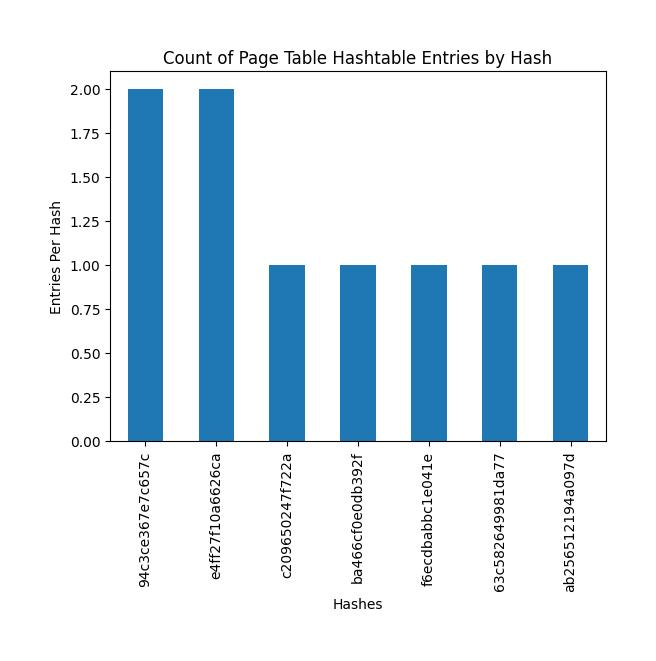
\includegraphics[width=0.5\textwidth]{images/m2_histogram.jpg}
    \caption{Hash table distribution.}
    \label{figure:m2_histogram}
\end{wrapfigure}
\\\\
We painfully recognize in hindsight that using a hash table as an ``optimization" for the overall search-time during a mapping/unmapping operation may not have been as fruitful as we anticipated, due to the sparsity of a process' virtual address space. It is generally the case that large portions of a process's virtual address space, at any given time, don't actually contain data that needs to be stored or processed. This was observed after running one of our test cases which mapped 1,000 arbitrary frames. Although our hash table's distribution was good (Figure \ref{figure:m2_histogram}), it contained only six entries following the mappings. If we had alternatively just stored page tables in a linked list, the search for a free virtual address region would remain the dominating contributor to speed. Put another way, when mapping frames we always must perform a relatively slow search through the linked list of regions in order to find a free space. The overall runtime of a mapping request would not be significantly reduced in the process of searching through an additional few page table nodes stored in a separate linked list. Going with a simpler implementation here would certainly have saved us a few headaches and we figured that we should have more carefully considered whether or not our optimization strategy would have had an observable effect. 

\subsection{Heap Memory Management}\label{m2-4}
In order for processes to freely allocate variable-sized portions of memory, we need to provide a mechanism through which it can access its heap. This is done primarily through a lazy allocation/mapping strategy which is orchestrated through the page fault handler.
\\\\
When a process requests memory from a system that is using lazy allocation, the entire virtual address region is reserved. However, the physical memory allocation and its mapping to any part of that reserved virtual region is only done when the memory is actually accessed. This has a few benefits, for example:
\begin{itemize}[itemsep=0pt]
    \item \textbf{More efficient memory usage}: Physical memory resources are allocated only at the last possible moment, preventing unnecessary allocations of large physical memory blocks that might never be fully used.
    \item \textbf{Reduced initial overhead}: The costs of physical memory allocation and mapping are deferred until later, which is especially helpful in cases where the memory requirements of the requesting process are not initially known.
    \item \textbf{Quicker process spawns}: Lazy allocation makes it unnecessary for a process to physically back all of its heap memory on startup, improving the spawn time.
    \item \textbf{Support for sparsity}: Applications that request large physical chunks of memory, but only use small portions of it are better handled.
\end{itemize}
In order to implement this, we define a specific region of a process's virtual address space as the heap. The page fault handler can only map within this region, and any physical frame that does not make up parts of the heap are not mapped by the fault handler. This introduces the assumption that the only lazily allocated memory is the heap. If we do not make this assumption, then we would need further mechanisms to determine what addresses the page fault handler is allowed to map and to distinguish between addresses belonging to the heap and to other memory regions.
\\\\
As described previously, our virtual memory allocator, in addition to the basic fields provided by its generic interface, distinguishes between ``reserved" and ``mapped" regions. Every mapping is associated with a mapping capability and thus we indicate whether or not a region is mapped by whether or not it holds one or more non-\texttt{NULL} mapping capabilities.
\\\\
When a process tries to access unmapped memory in the heap, a page fault is raised, where control is then handed over to the page fault handler which validates the source of the fault. This includes checking if the accessed address lies within the heap, if the access type is appropriate (read, write, or execute), whether or not we're dereferencing a \texttt{NULL} pointer, and so on. Once the page fault is verified to be a valid virtual memory access, we allocate a page of physical RAM and map it to a page-aligned address containing the faulting address. 

\subsection{Performance Measurements}
Timing measurements were done using the \texttt{time} system call from \texttt{time.h} and then exported and plotted using \texttt{matplotlib}.
\begin{itemize}[itemsep=0pt]
    \item \textbf{Figure \ref{figure:paging_map_small_frame_scatter}}: We evaluated the latency of mapping a series of small frames (1 page each). The average latency increases by only a small margin. Note that there is a second, less dense band of slower latencies above the main band. We suspect that these cases occur when one or more new levels of the page table need to be allocated.
    \begin{figure}[ht]
        \centering
        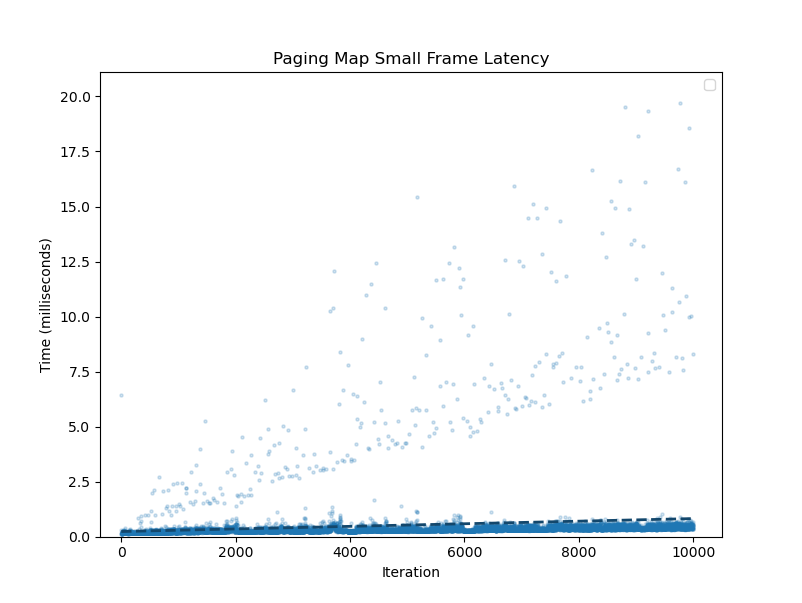
\includegraphics[width=0.58\columnwidth]{images/paging_map_small_frame_scatter.png}
        \caption{Mapping a series of 1-page frames.}
        \label{figure:paging_map_small_frame_scatter}
    \end{figure}
    \item \textbf{Figure \ref{figure:paging_map_large_frame_scatter}}: We evaluated the latency of mapping a series of large frames (100 pages each). There is a higher density in the second band compared to our small-frame-mapping test since a larger ratio of requests result in the creation and mapping of new VNodes. The per-iteration increase in latency is still small which may indicate that hash tables are effective for efficient VNode accesses.
    \begin{figure}[ht]
        \centering
        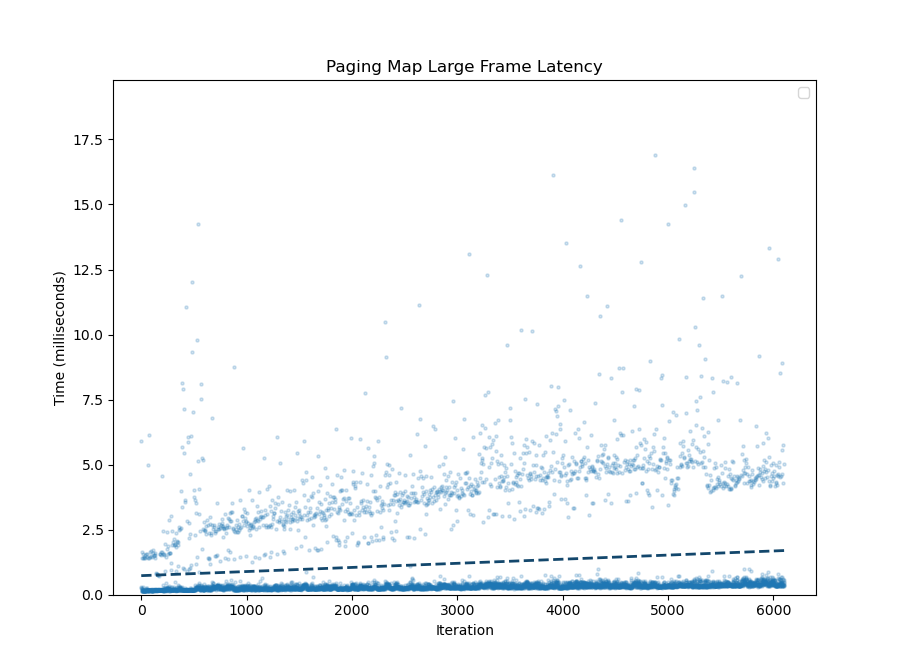
\includegraphics[width=0.58\columnwidth]{images/paging_map_large_frame_scatter.png}
        \caption{Mapping a series of 100-page frames.}
        \label{figure:paging_map_large_frame_scatter}
    \end{figure}
    \item \textbf{Figure \ref{figure:malloc_scatter}}: We evaluate our \texttt{malloc} implementation by allocating a large array and then causing page faults by accessing new pages on each iteration. The latency appears to grow linearly which falls in line with the linear growth of memory manager allocations and paging frame mappings. The latency surpasses 2ms after 5,000 page faults which is less than ideal and may require revisiting our generic allocator implementation should it become a bottleneck.
    \begin{figure}[ht]
        \centering
        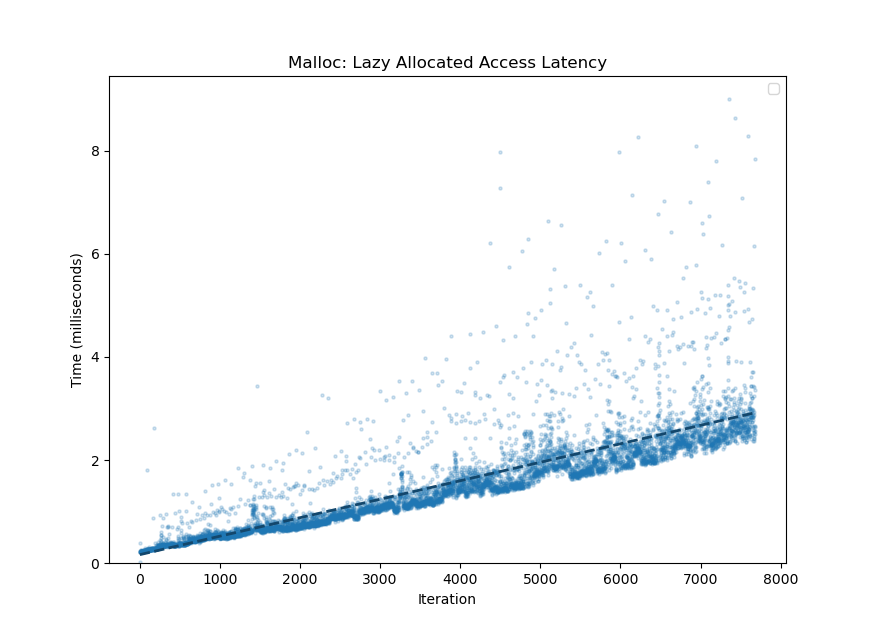
\includegraphics[width=0.58\columnwidth]{images/malloc_scatter.png}
        \caption{Page accesses in a lazy-allocated memory chunk.}
        \label{figure:malloc_scatter}
    \end{figure}
\end{itemize}
